%\PassOptionsToPackage{english}{babel}
% \RequirePackage{fix-cm}
\documentclass[final,t]{beamer}
\usefonttheme{professionalfonts}
\mode<presentation>
{
%  \usetheme{Warsaw}
%  \usetheme{Aachen}
%  \usetheme{Oldi6}
%  \usetheme{I6td}
  \usetheme{I6dv}
%  \usetheme{I6pd}
%  \usetheme{I6pd2}
}
% additional settings
\setbeamerfont{itemize}{size=\normalsize}
\setbeamerfont{itemize/enumerate body}{size=\normalsize}
\setbeamerfont{itemize/enumerate subbody}{size=\normalsize}

\usepackage{xfrac}
\usepackage{mathrsfs}

\DeclareFontFamily{U}{rsfs}{\skewchar\font127 }
\DeclareFontShape{U}{rsfs}{m}{n}{%
   <-6> rsfs5
   <6-8> rsfs7
   <8-> rsfs10
}{}

\usepackage{algorithm}
% \usepackage{algorithmic}
\usepackage[noend]{algpseudocode}


\usepackage{Definitions}
\usepackage{tensor}
\usepackage{empheq}
\usepackage{array}
% \usepackage{color}
% \usepackage[usenames,dvipsnames,svgnames,table]{xcolor}
% \usepackage{tikz}
% \usetikzlibrary{calc}

% additional packages
\usepackage{times}
\usepackage{amsmath,amsthm, amssymb, latexsym}
\usepackage{exscale}

\usepackage{graphicx} % more modern
\usepackage{wrapfig}
% \usepackage{subfigure}
% \usepackage{caption}

% \boldmath
\usepackage{booktabs, array}
% \usepackage{rotating} %sideways environment
\usepackage[english]{babel}
\usepackage[latin1]{inputenc}
\usepackage[orientation=landscape,size=custom,width=155,height=90,scale=1.4]{beamerposter}
\listfiles
\graphicspath{{figure/}}


\newenvironment<>{thmblock}[2][1\textwidth]{%
  \setlength{\textwidth}{#1}
\setbeamertemplate{blocks}[rounded][shadow=true]
  \begin{actionenv}#3%
    \def\insertblocktitle{#2}%
    \par%
    \usebeamertemplate{block begin}}
  {\par%
    \usebeamertemplate{block end}%
  \end{actionenv}}

\newcommand{\algabb}{BASE}

\title{\VERYHuge 
Nonparametric Iterative Machine Teaching\\}

\author{ \Large
  Chen Zhang$^1$, Xiaofeng Cao$^1$, Weiyang Liu$^{2,3}$, Ivor W. Tsang$^{4}$, James T. Kwok$^{5}$
}

% abbreviations
\usepackage{xspace}
\makeatletter
\DeclareRobustCommand\onedot{\futurelet\@let@token\@onedot}
\def\@onedot{\ifx\@let@token.\else.\null\fi\xspace}
\makeatother

\begin{document}
\begin{frame}
\vspace{-0.4in}
\begin{columns}[t]

%======================First coloumn
\begin{column}{.27\linewidth}
%-----------------block 1---------------
\begin{block}{Machine Teaching}
Machine teaching (MT) is the study of how to design the \alert{optimal teaching set}, typically with \alert{minimal} examples, so that learners can quickly learn \alert{target models} based on these examples.

\vspace{6mm}

It can be considered an \alert{inverse problem} of machine learning, where machine learning aims to learn model parameters from a dataset, while MT aims to find a minimal dataset from the target model parameters.

\vspace{6mm}

Considering the \alert{interaction manner} between teachers and learners, MT can be conducted in either\begin{itemize}
    \item {\color{blue} batch} fashion where the teacher is allowed to interact with the learner once, or 
    \item {\color{blue} iterative} fashion where an iterative teacher would feed examples sequentially based on current status of the iterative learner.
\end{itemize}
\end{block}

%-----------------block 2---------------
\begin{block}{Motivation}

\begin{wrapfigure}{R}{0.5\textwidth}
  \centering
  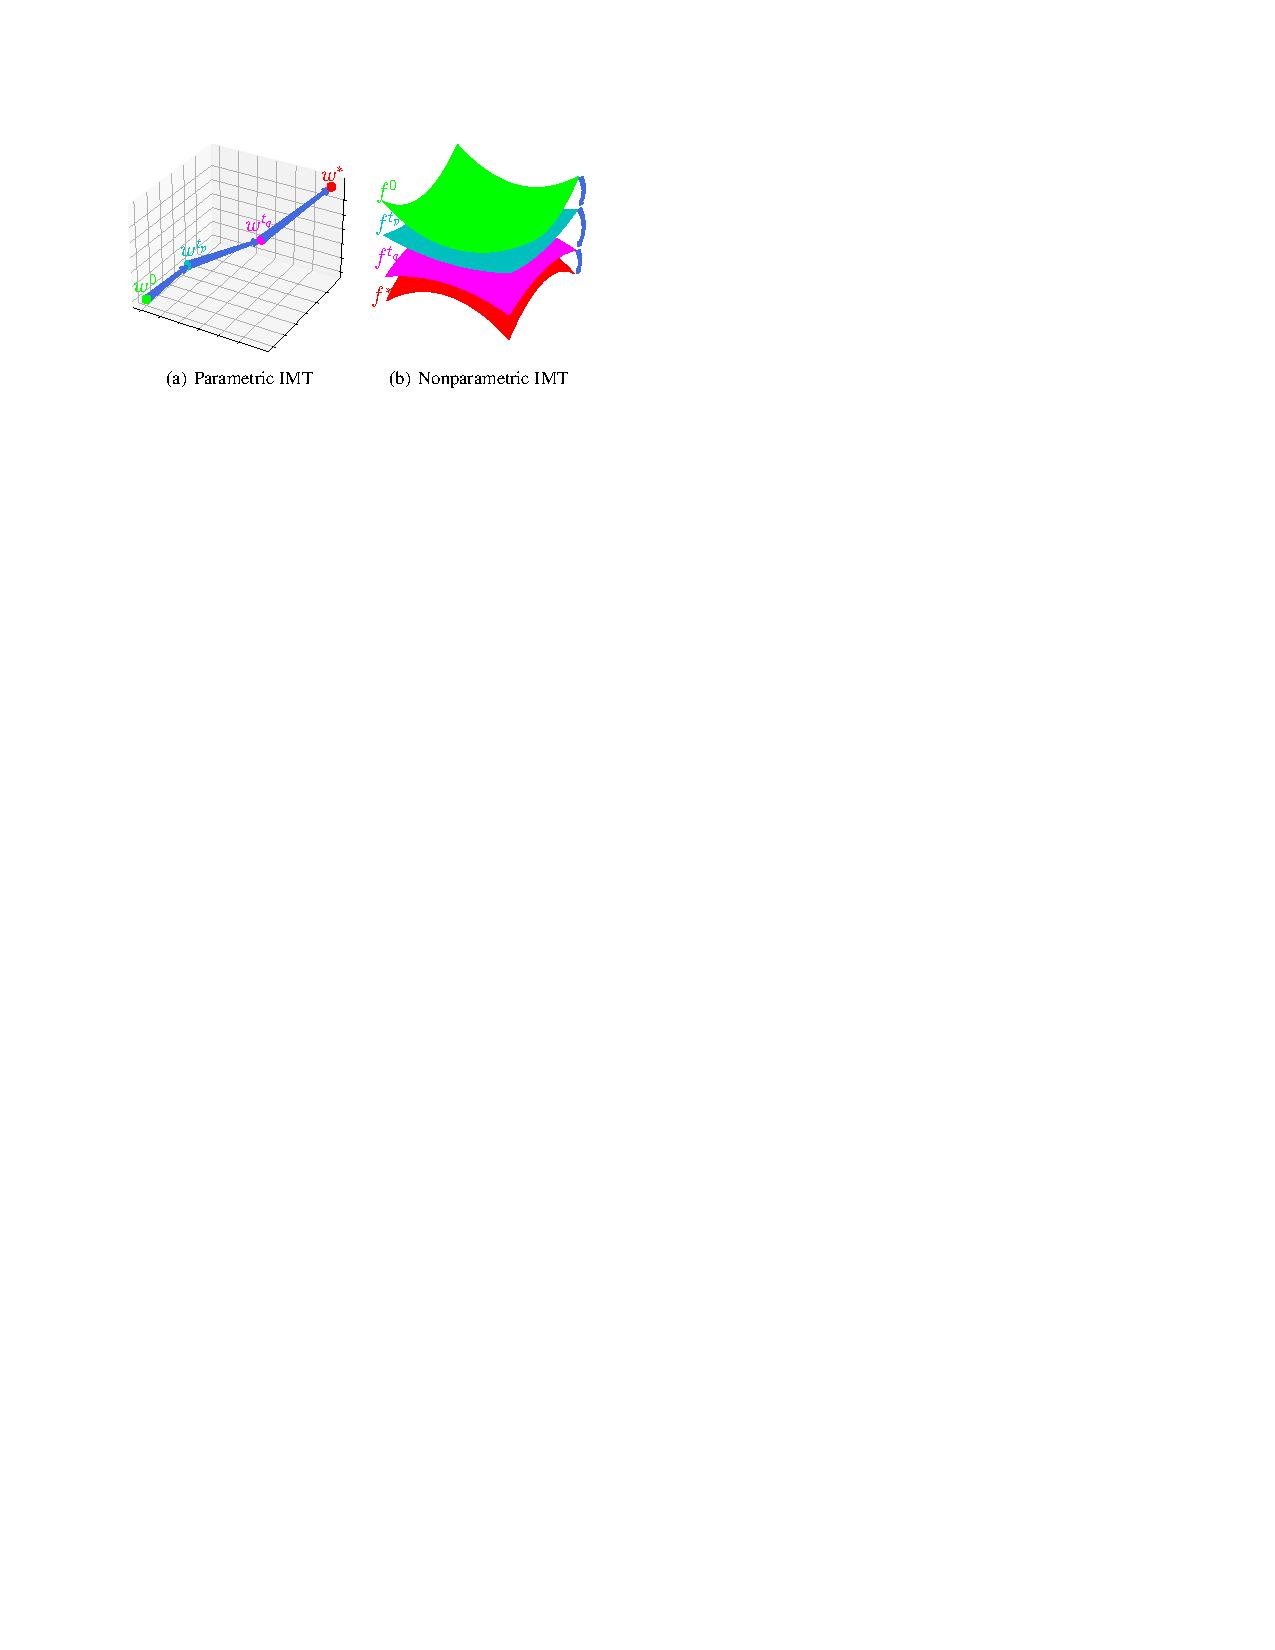
\includegraphics[width=0.44\textwidth]{comp.pdf}
  \caption{\footnotesize Comparison between parameterized and nonparametric IMT.}
  \label{fig}
\end{wrapfigure}

Previous iterative machine teaching algorithms are solely based on \alert{parameterized} families of target models. They mainly focus on convergence in the parameter space, resulting in difficulty when the target models are defined to be \alert{functions without dependency on parameters}. To address such a limitation, we study a more general task -- {\bf Nonparametric Iterative Machine Teaching}, which aims to teach {\color{red} nonparametric target models} to learners in an iterative fashion.

\vspace{6mm}
      {\bf \color{blue} Main Contribution}: 
\begin{itemize}
\item We comprehensively study {\bf Nonparametric Iterative Machine Teaching}, which focuses on exploring iterative algorithms for teaching \alert{parameter-free target models} from the \alert{optimization} perspective.
\item We propose two teaching algorithms, which are named \alert{Random Functional Teaching} (RFT) and \alert{Greedy Functional Teaching} (GFT), respectively. RFT is based on random sampling with ground truth labels, and the derivation of GFT is based on the maximization of an informative scalar.
\item We theoretically analyze the \alert{asymptotic behavior} of both RFT and GFT. We prove that per-iteration reduction of loss $\mathcal{L}$ for RFT and GFT has a \alert{negative upper bound} expressed by the discrepancy of iterative teaching, and we derive that the iterative teaching dimension (ITD) of GFT is $\mathcal{O}(\psi(\frac{2\mathcal{L}(f^0)}{\tilde{\eta}\epsilon}))$, which is shown to be lower than the ITD of RFT, $\mathcal{O}(2\mathcal{L}(f^0)/\left(\tilde{\eta}\epsilon\right))$.
\end{itemize}
\vspace{-7mm}
\end{block}
\end{column}


%======================Second coloumn
\begin{column}{.37\linewidth}
%-----------------block 1---------------
\begin{block}{Teaching Settings}
{\bf \color{blue} Functional Optimization}: We define nonparametric iterative machine teaching as a \alert{functional minimization} over the collection of potential teaching sequences $\mathbb{D}$ in the reproducing kernel Hilbert space:
\begin{equation}\label{eq1}
 \mathcal{D}^*=\underset{\mathcal{D}\in\mathbb{D}}{\arg\min}\quad \mathcal{M}(\hat{f},f^*)+\lambda\cdot \text{len}(\mathcal{D}) \qquad\text{s.t.}\quad\hat{f}=\mathcal{A}(\mathcal{D}),
\end{equation}
where $\mathcal{M}$ denotes a discrepancy measure, $\text{len}(\mathcal{D})$, 
which is regularized by a constant $\lambda$, is the length of the teaching sequence $\mathcal{D}$, and $\mathcal{A}$ represents the learning algorithm of learners. 


\end{block}

%-----------------block 2---------------
\begin{block}{Functional Teaching Algorithms}
\centering
\vspace{-1cm}
\begin{tabular}{ccc}
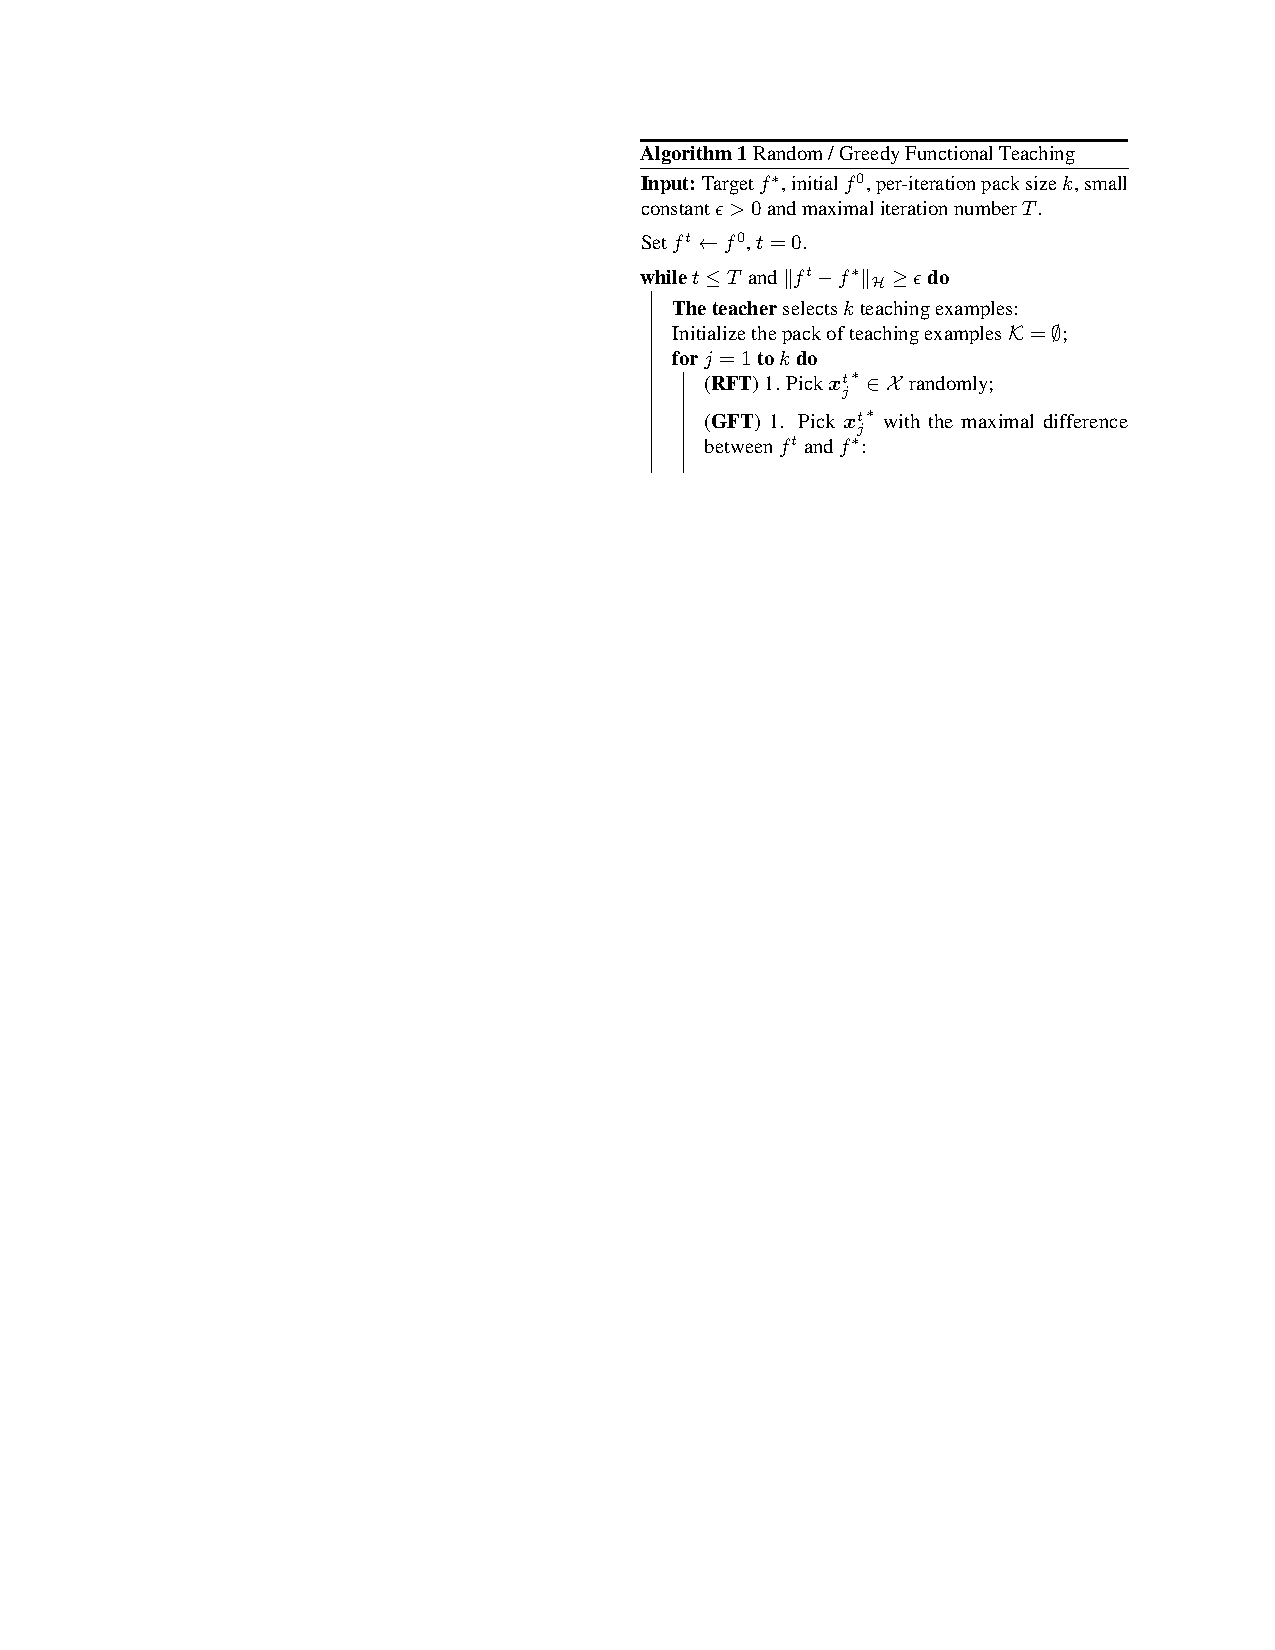
\includegraphics[width=0.5\textwidth]{algo1.pdf}

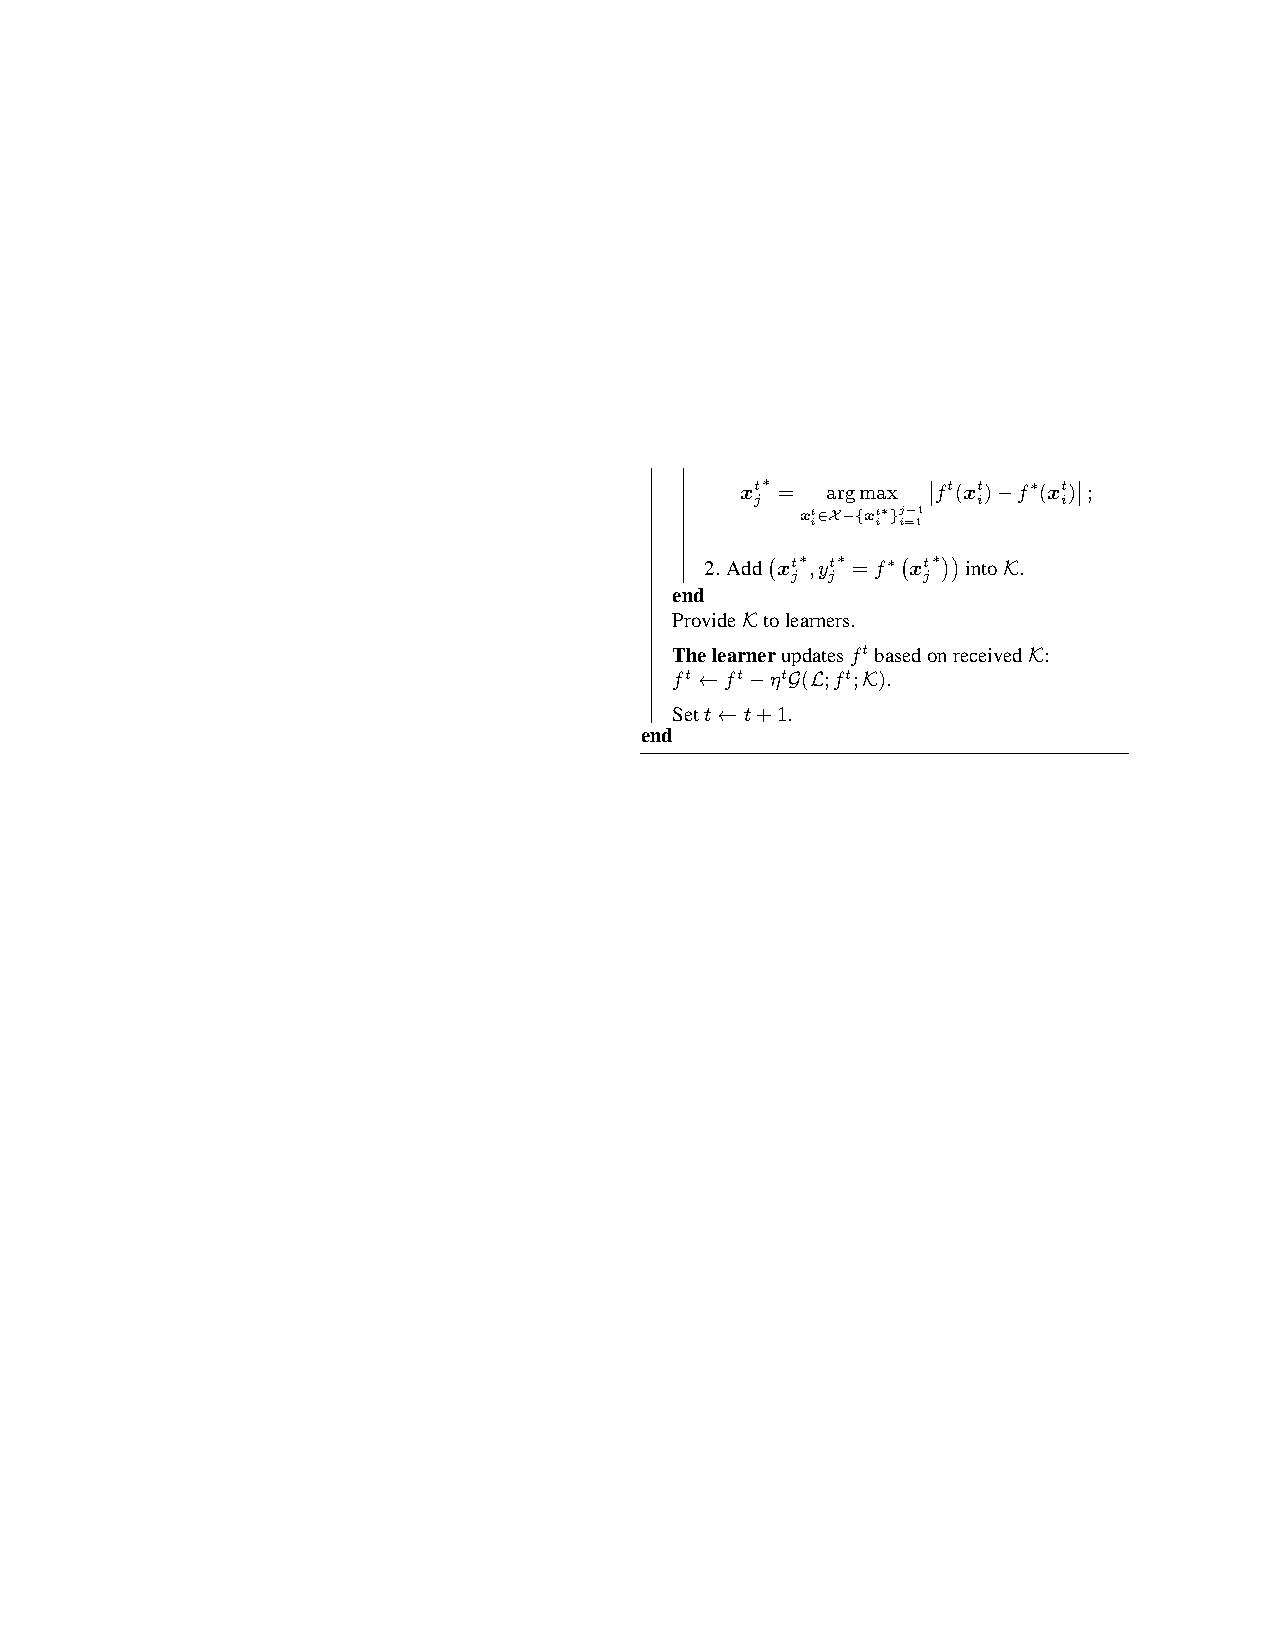
\includegraphics[width=0.5\textwidth]{algo2.pdf}\vspace{-1mm}
\\
\end{tabular}
\vspace{-1cm}
\end{block}

%-----------------block 3---------------
\begin{block}{Analysis of Iterative Teaching Dimension}
\textbf{Assumption 1}. The loss function $\mathcal{L}(f)$ is $L_\mathcal{L}$-Lipschitz smooth, \ie, $\forall f,f'\in\mathcal{H}$ and $\bm{x}\in\mathcal{X}$ $$\left|E_{\bm{x}}\left[\nabla_f \mathcal{L}(f)\right]-E_{\bm{x}}\left[\nabla_f\mathcal{L}(f')\right]\right|\leq L_\mathcal{L} \left|E_{\bm{x}}\left[f\right]-E_{\bm{x}}\left[f'\right]\right|, $$ where $L_\mathcal{L}\geq0$ is a constant.

\vspace{6mm}

\textbf{Assumption 2}. The kernel function $K(\bm{x},\bm{x}')\in\mathcal{H}$ is bounded, \ie, $\forall \bm{x},\bm{x}' \in\mathcal{X},\,K(\bm{x},\bm{x}')\leq M_K$, where $M_K\geq0$ is a constant.

\vspace{6mm}

\textbf{Lemma 3} (Sufficient Descent for \textbf{RFT}). Under Assumption 1 and 2, if $\eta^t\leq 1/(2L_\mathcal{L}\cdot M_K)$, RFT teachers can \alert{reduce the loss} $\mathcal{L}$ by $\mathcal{L}(f^{t+1})-\mathcal{L}(f^t)\leq-\eta^t/2\cdot\mathbb{S}_{\mathcal{L}}(f^t;{\bm{x}^t})$.

\vspace{6mm}

\textbf{Theorem 4} (Convergence for \textbf{RFT}). Suppose the model of learners is initialized with $f^0\in\mathcal{H}$ and returns $f^t\in\mathcal{H}$ after $t$ iterations, we have the \alert{upper bound of minimal $\mathbb{S}_{\mathcal{L}}(f^t;{\bm{x}^t})$} as $\min_t\mathbb{S}_{\mathcal{L}}(f^t;{\bm{x}^t}) \leq2\mathcal{L}(f^0)/\left(\tilde{\eta}t\right)$,
	where $0<\tilde{\eta}=\underset{t}{\min}\,\eta^t\leq \frac{1}{2L_\mathcal{L}\cdot M_K}$.

\vspace{6mm}

\textbf{Lemma 5} (Sufficient Descent for \textbf{GFT}). Under Assumption 1 and 2, if $\eta^t\leq 1/(2L_\mathcal{L}\cdot M_K)$, GFT teachers can reduce the loss $\mathcal{L}$ at a \alert{faster speed}, 
$\mathcal{L}(f^{t+1})-\mathcal{L}(f^t)\leq-\eta^t/2\cdot\mathbb{S}_{\mathcal{L}}(f^t;{\bm{x}^t}^*)\leq-\eta^t/2\cdot\mathbb{S}_{\mathcal{L}}(f^t;{\bm{x}^t})$.

\vspace{6mm}

\textbf{Theorem 6} (Convergence for \textbf{GFT}). Suppose the model of learners is initialized with $f^0\in\mathcal{H}$ and returns $f^t\in\mathcal{H}$ after $t$ iterations, we have the \alert{upper bound of minimal $\mathbb{S}_{\mathcal{L}}(f^t;{\bm{x}^j}^*)$} as $\min_j\mathbb{S}_{\mathcal{L}}(f^j;{\bm{x}^j}^*)\leq\frac{2}{\tilde{\eta}\psi(t)}\mathcal{L}(f^0)$, where $0<\tilde{\eta}=\underset{t}{\min}\,\eta^t\leq \frac{1}{2L_\mathcal{L}\cdot M_K}$, $\psi(t)=\sum_{j=0}^{t-1}\gamma^j$ and $\gamma^j = \frac{\mathbb{S}_{\mathcal{L}}(f^j;{\bm{x}^j})}{\mathbb{S}_{\mathcal{L}}(f^j;{\bm{x}^j}^*)}\in(0,1]$ named greedy ratio.

\end{block}
      
\end{column}


%======================Third coloumn
\begin{column}{0.28\linewidth}
\begin{block}{Experiments and Results}

\begin{itemize}
    \item {\bf Synthetic data.}
\end{itemize}

\centering
\vspace{6mm}
\begin{tabular}{lclc}
{\color{blue} 1D Gaussian Mixture.} \vspace{-4mm}\\

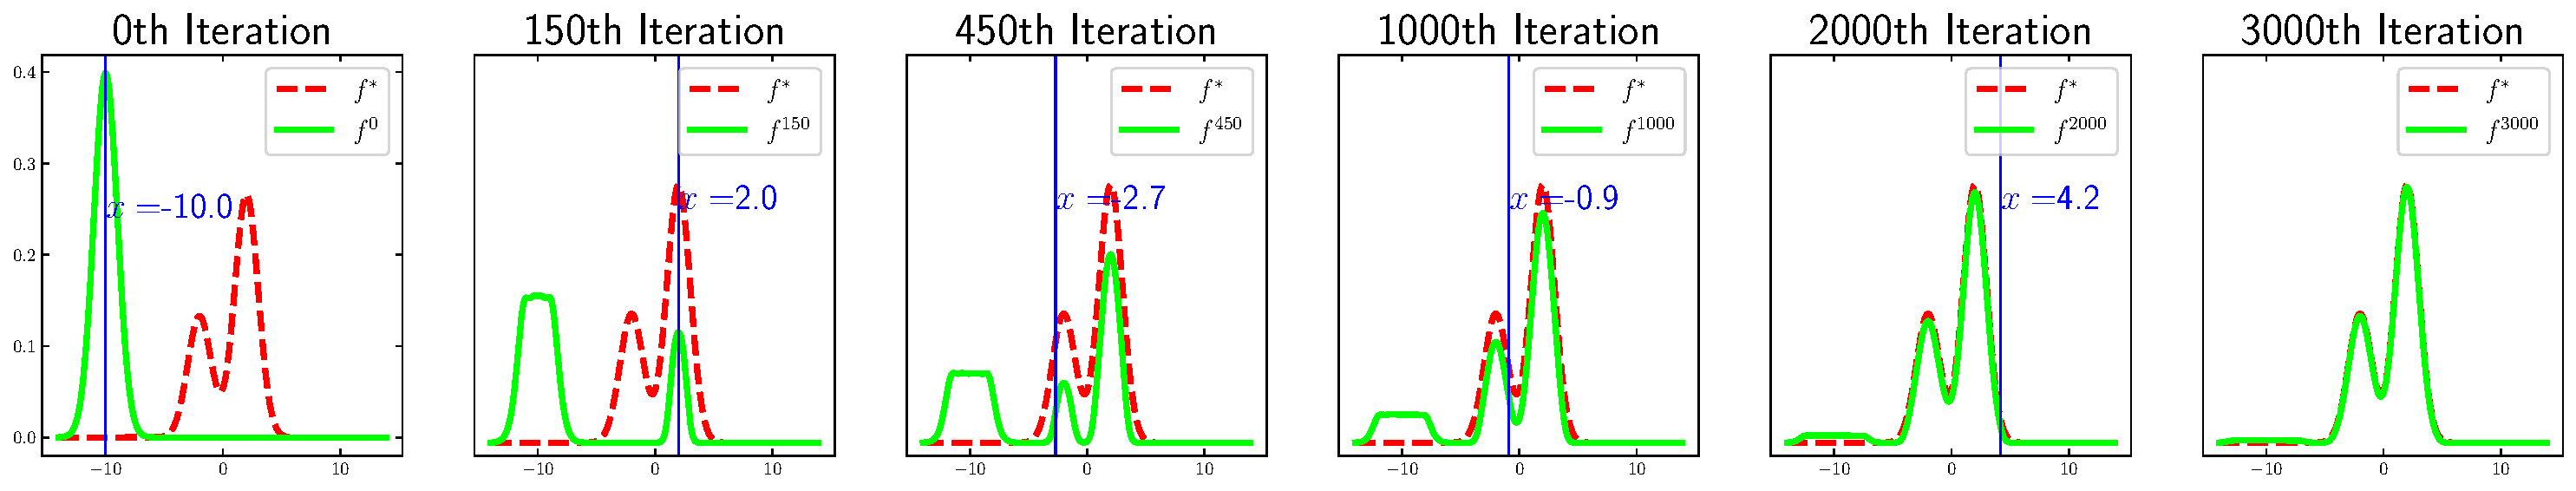
\includegraphics[width=\linewidth]{./out/toy/distribution}\\

{\color{blue} 2D Classification.}\vspace{-4mm}\\

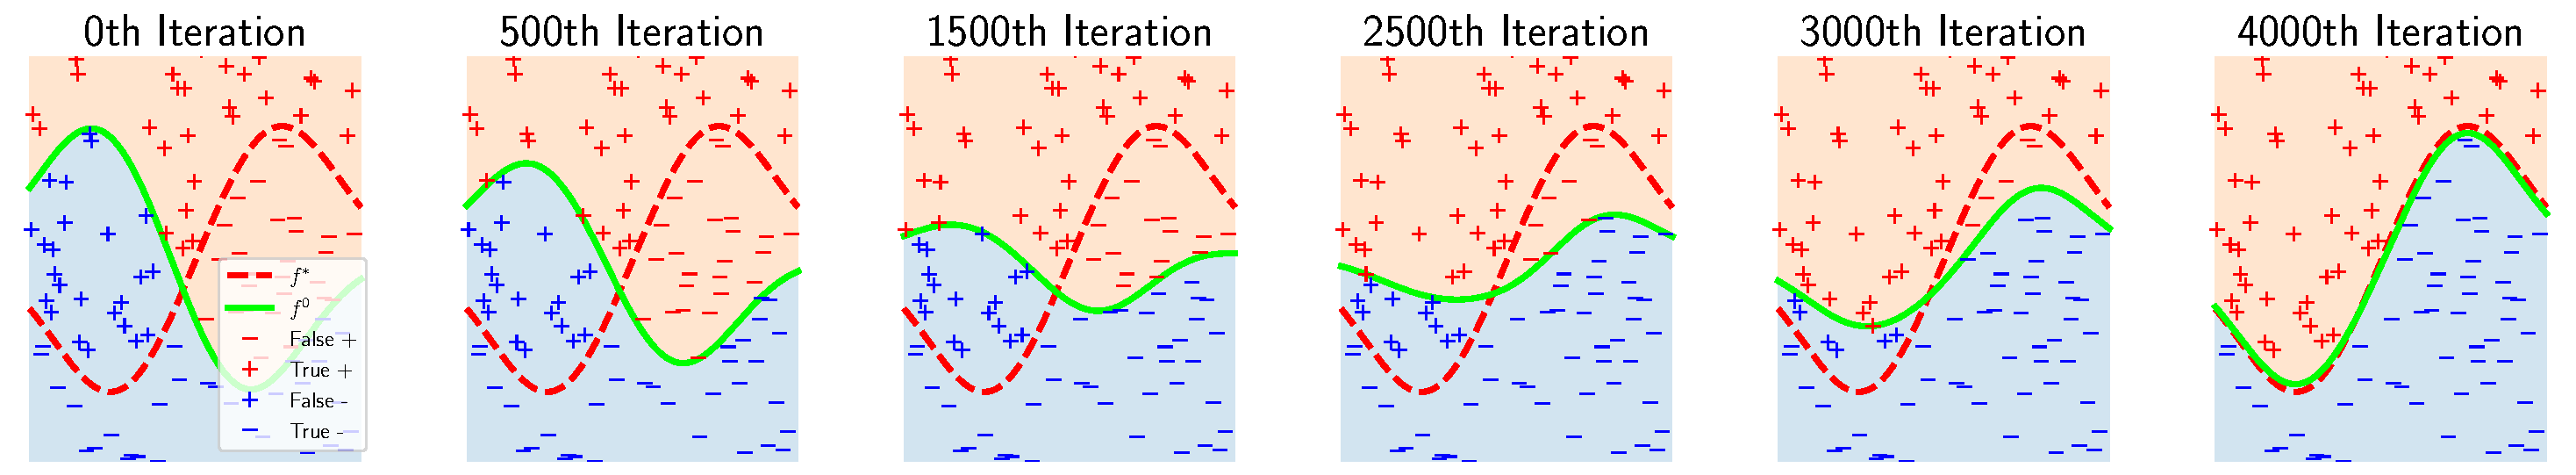
\includegraphics[width=\linewidth]{./out/toy/classification}
\end{tabular}

\vspace{12mm}

\begin{itemize}
    \item {\bf  Real-world data.}
\end{itemize}

\centering
\vspace{10mm}
\begin{tabular}{ccc}

{\color{blue} Digit Correction.} & & {\color{blue} Cheetah Impartation.}\vspace{-1mm}\\
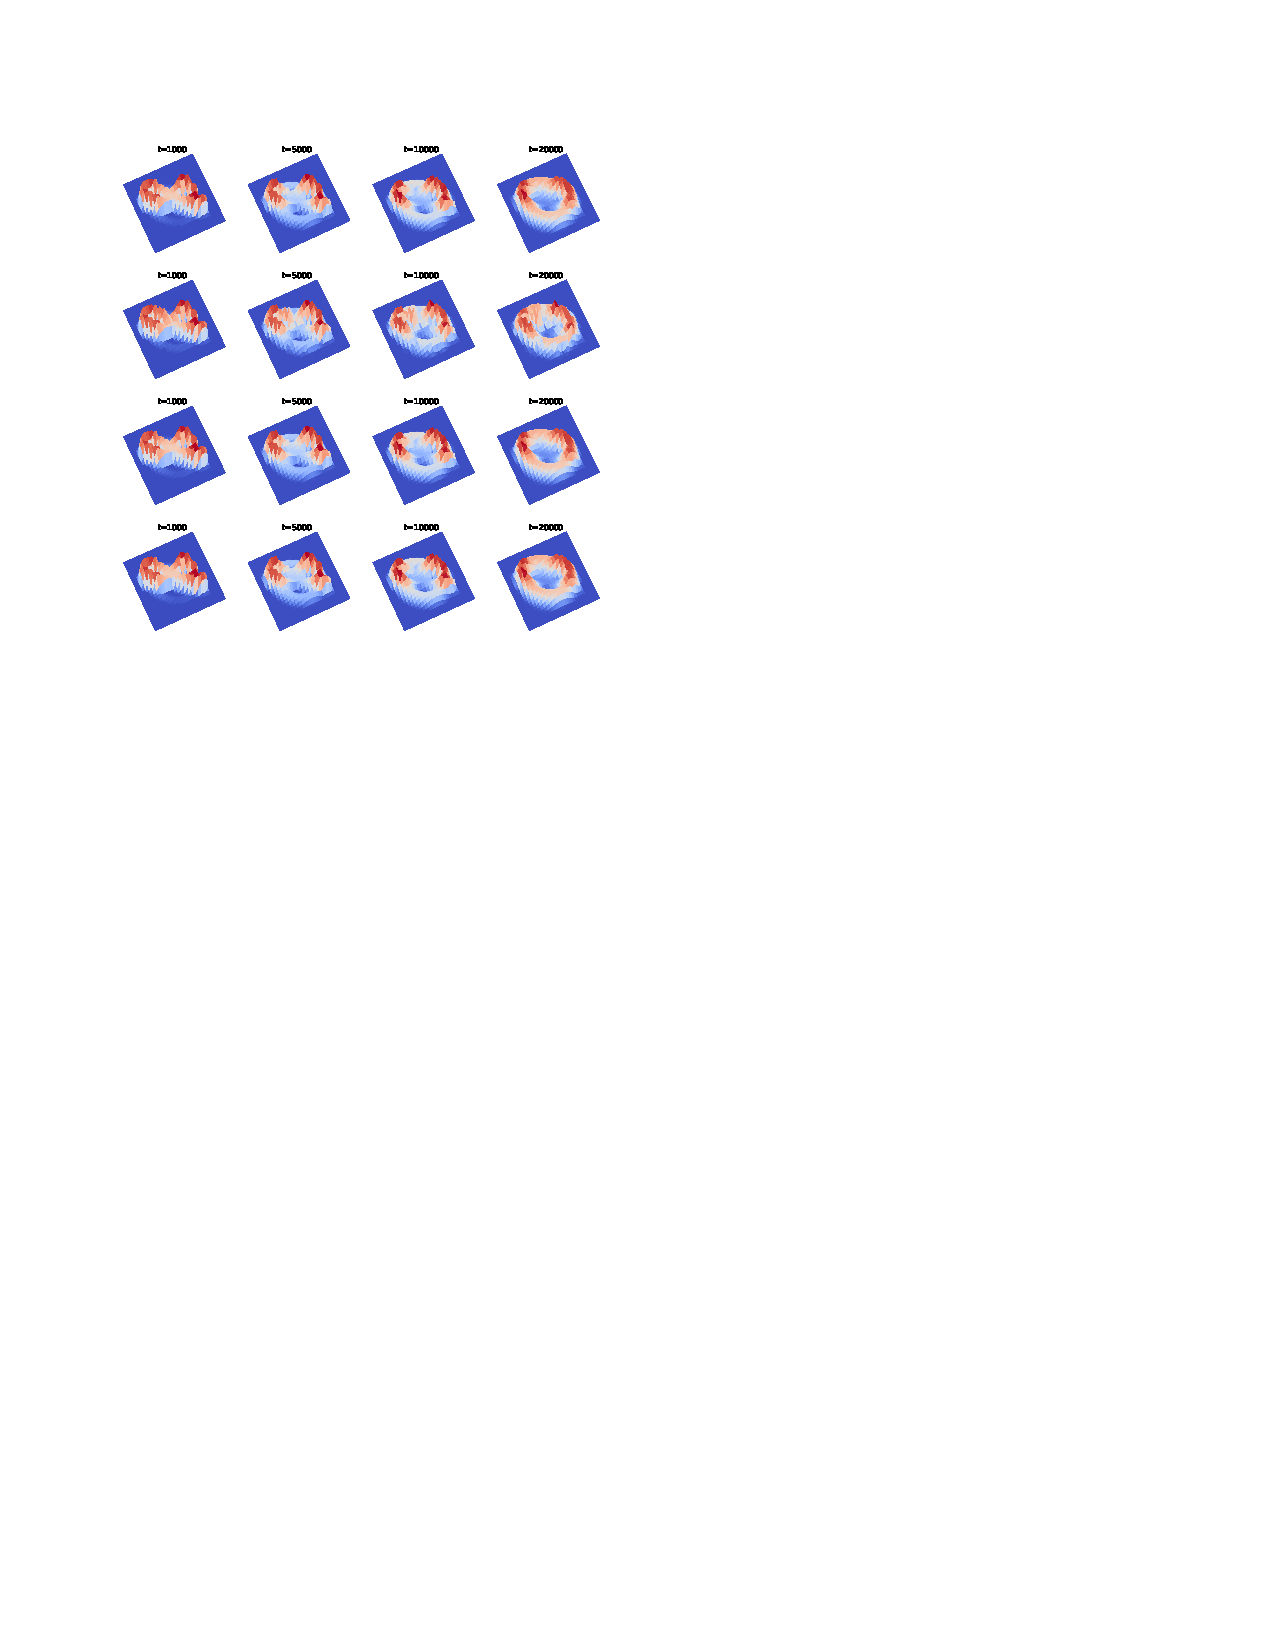
\includegraphics[width=0.5\textwidth]{./out/realworld/digit}\vspace{-1mm} & 

&
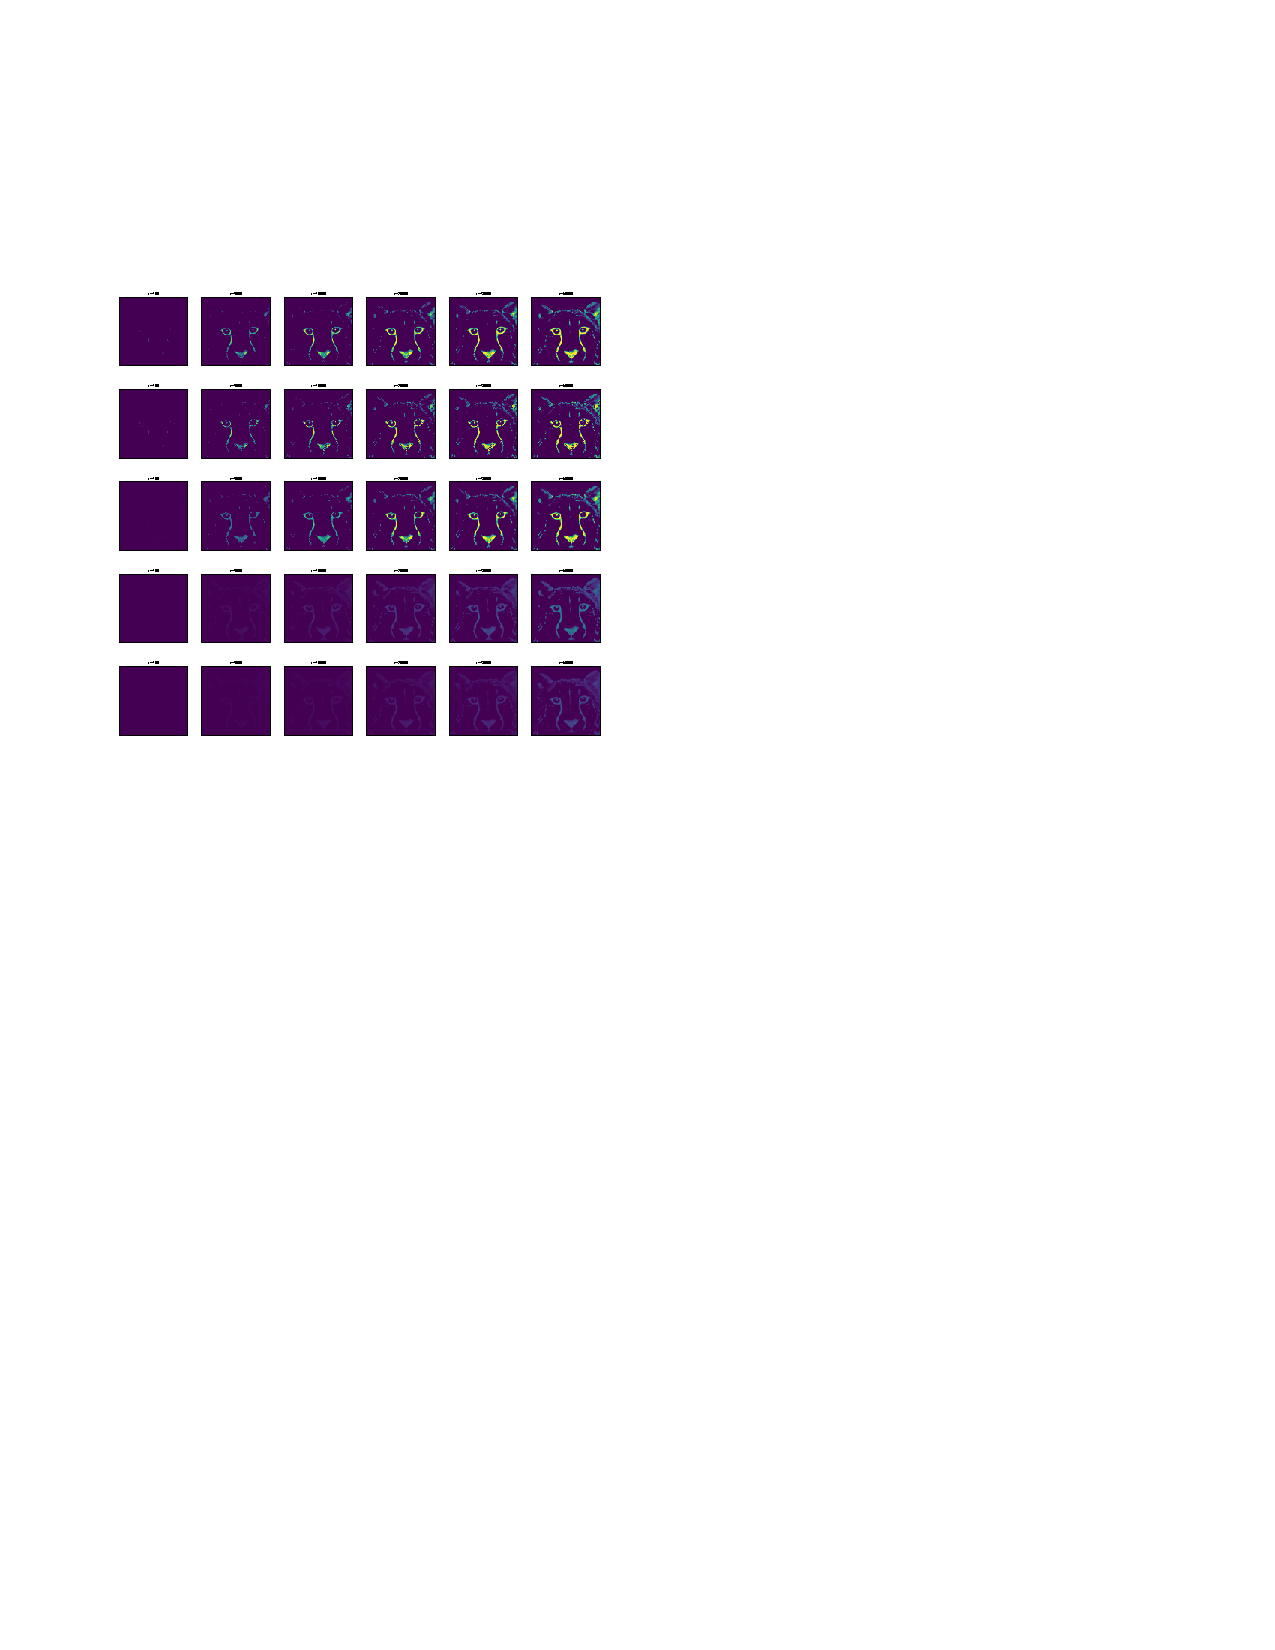
\includegraphics[width=0.5\textwidth]{./out/realworld/cheetah}
\end{tabular}

\vspace{6mm}

\begin{tabular}{lc}
{\color{blue} Sketch for Missing Person Report.}\vspace{-4mm}\\

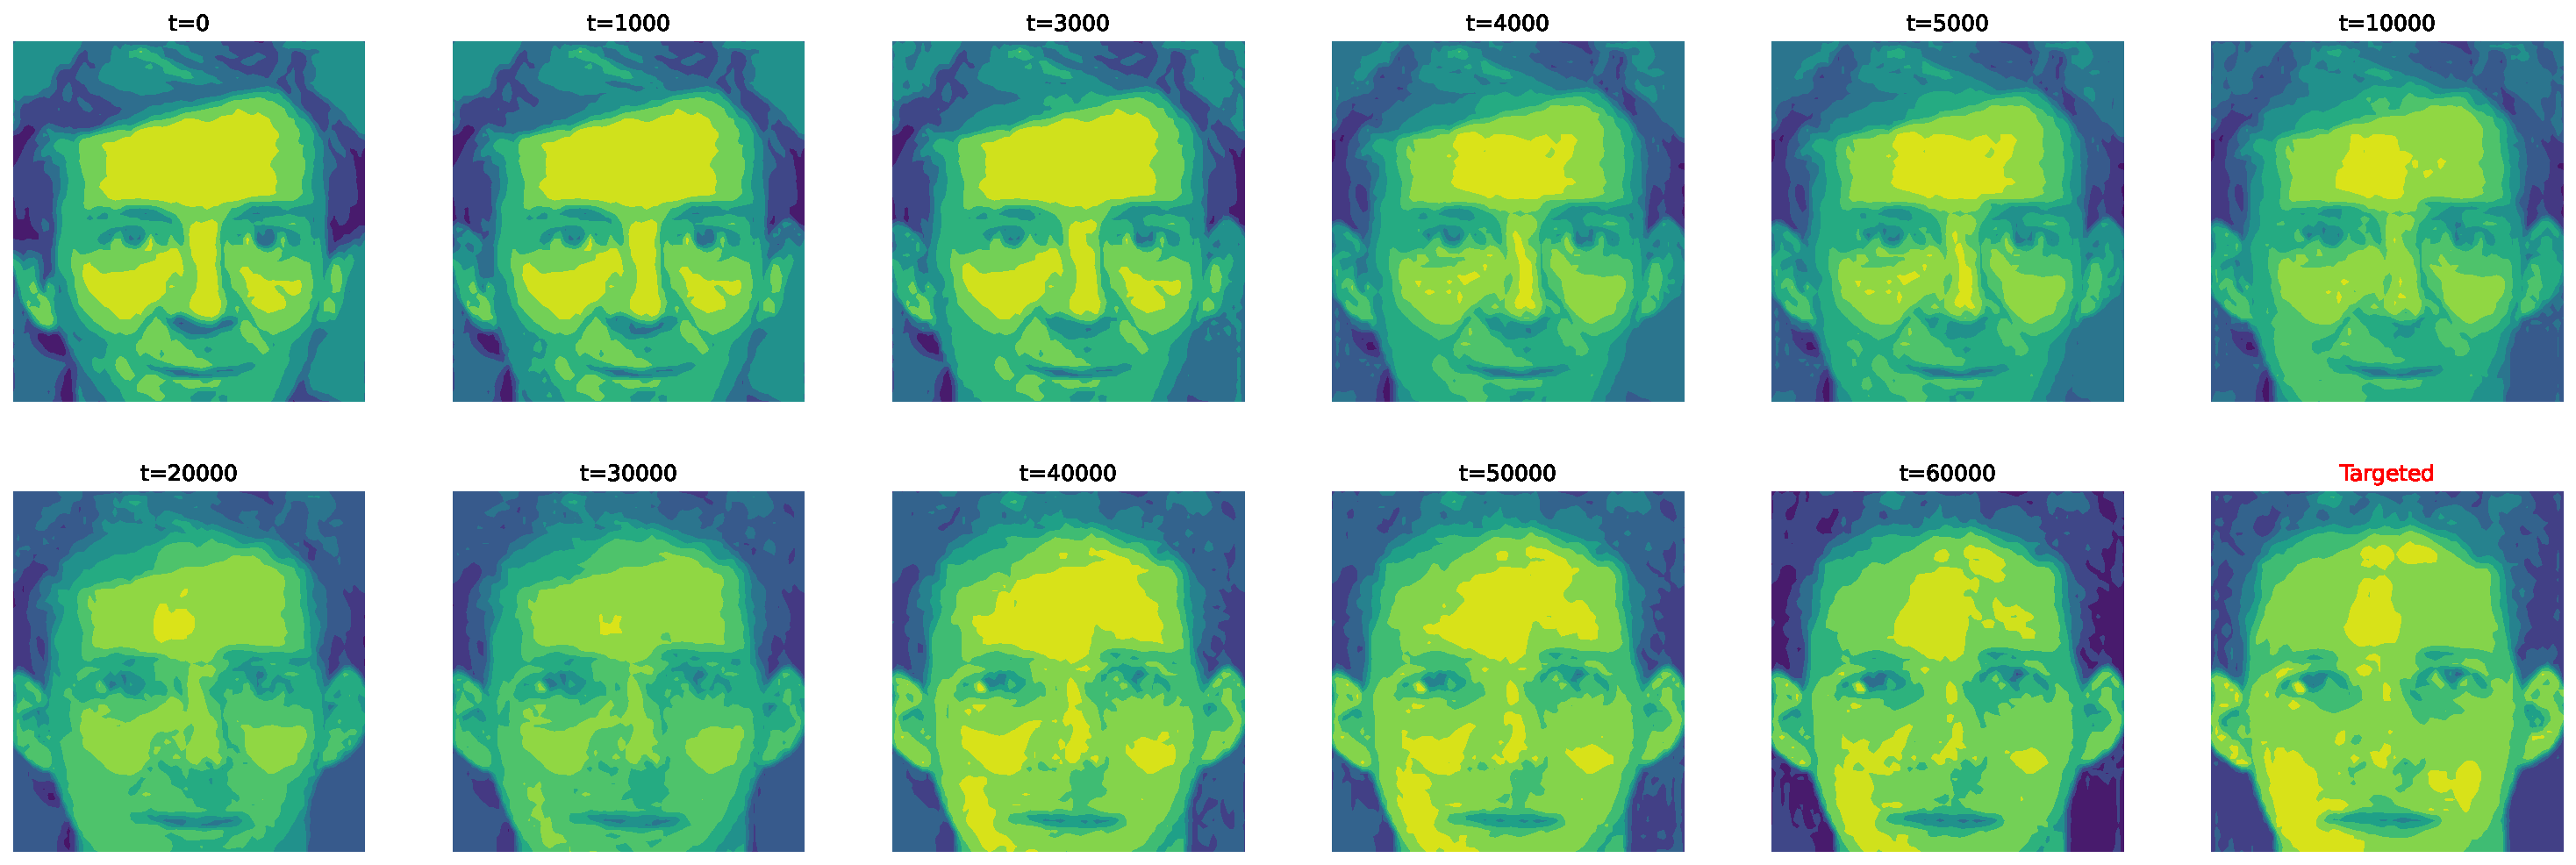
\includegraphics[width=\linewidth]{./out/realworld/2d face eta=0.05 B=one}

\end{tabular}

\end{block}

\end{column}

\end{columns}
\end{frame}

\end{document}

%%%%%%%%%%%%%%%%%%%%%%%%%%%%%%%%%%%%%%%%%%%%%%%%%%%%%%%%%%%%%%%%%%%%%%%%%%%%%%%%%%%%%%%%%%%%%%%%%%%%
%%% Local Variables: 
%%% mode: latex
%%% TeX-PDF-mode: t
%%% End: 